\begin{center}
  \textbf{Отчёт лабораторной работы №\envReportLabNumber}
\end{center}

\textbf{Тема}:
<<\envReportTitle>>

\textbf{Цель}:
изучить основы анализа, обработки и прогнозирования временных рядов,
приобрести навыки работы с методами анализа,
обработки и прогнозирования временных рядов в системе STATISTICA StatSoft,
осуществить обработку, анализ и прогнозирование ряда и интерпретацию результатов.

% = = = = = = = = = = = = = = = =

\phantomsection
\addcontentsline{toc}{section}{Подготовка к лабораторной работе}

\begin{center}
  \textbf{Подготовка к лабораторной работе}
\end{center}

В связи с тем, что в лабораторной работе нужно использовать программу <<Statistica 10>>,
а она под операционную систему WinXP-Win7,
а у меня основная ОС Ubuntu 22.04,
то я установлю виртуальную машину Windows XP.

В связи с тем, что ISO WinXP нельзя скачать с серверов Microsoft, то прийдется качать через торрент \cite{TorrentWinXP}.
Жаль что нет свободной версии (open source) Windows и с безвыходном положении приходится качать с левого сайта.
Торрент буду качать через open source программу qBitTorrent \cite{downloadQBitTorrent}.

Подключать ISO образ WinXP буду к виртуальной машине.
В качестве виртуальной машины буду использовать программу Oracle Virtual Box \cite{downloadVirtualBox}.

Чтобы запустить <<Statistica 10>> я нашел на торрент трекере портабельную программу. 
Очень жаль что, пользуюсь проприетарным софтом, но у меня безвыходная ситуация.
Портабельная (переносимая) версия программы - это программа, которая не устанавливается в систему, не мусорит систему
и может запускаться с флешки.

Для работы <<Statistica 10>> на WinXp также нужно скачать Visual C++ 2008 \cite{downloadVisualCpp2008}.

Для передачи файлов в виртуальную машину, можно подключить общие папки,
либо скачивать все через браузер Firefox 52.9.0esr \cite{downloadFirefox5290esr}.

\begin{center}
  \textbf{Общие сведения}
\end{center}

Главная > Открыть > Series\_G.sta

Результат действий смотри на рисунке~\ref{fig:1}.

\begin{figure}[!h]
  \centering

  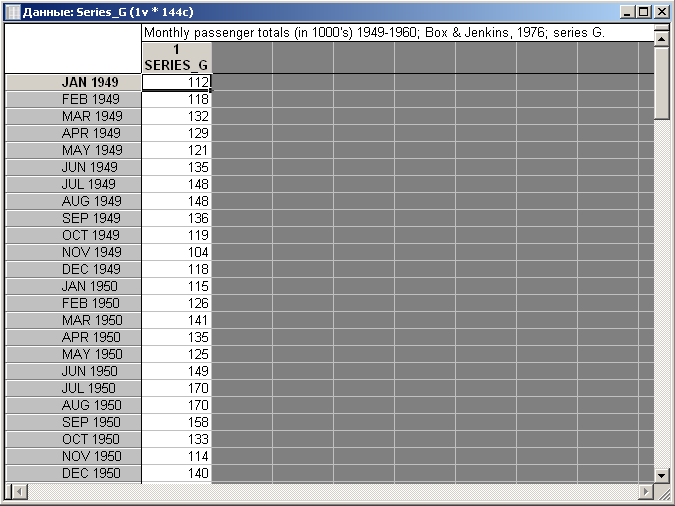
\includegraphics[height=6cm]
  {inc/Series_G/1.PNG}

  \caption{Общие сведения}

  \label{fig:1}
\end{figure}

\begin{center}
  \textbf{Определение анализа}
\end{center}

Анализ > Углубленные методы > Временные ряды и прогнозирование\\
> Переменные > ОК\\
> Методы > АРПСС и автокорреляционные функции > Методы

Результат действий смотри на рисунке~\ref{fig:2}.

\begin{figure}[!h]
  \centering

  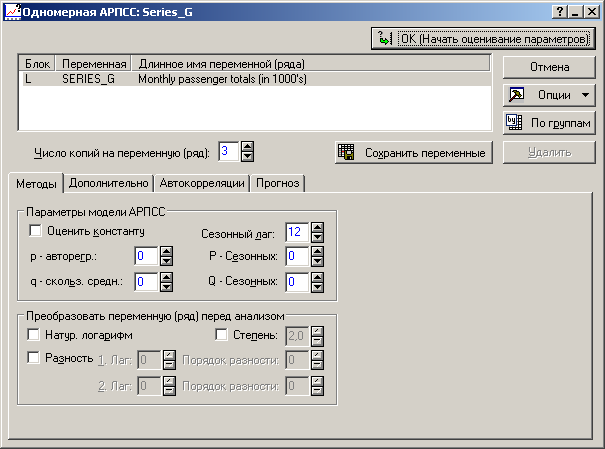
\includegraphics[height=6cm]
  {inc/Series_G/2.PNG}

  \caption{Определение анализа}

  \label{fig:2}
\end{figure}

\begin{center}
  \textbf{Фаза идентификации}
\end{center}

Анализ > Углубленные методы > Временные ряды и прогнозирование > Новый\\
> Переменные > ОК\\
> Методы > АРПСС и автокорреляционные функции > Методы \\
> Дополнительно > Другие преобразования и графики\\
> Графики\\
> Задать масштаб по оси Х (мин, знач, шаг) > 1 > 12\\
> Пометить точки по оси Х > Именами наблюдений\\
> График (рядом с кнопкой Просмотр выдел. Переменной)

Результат действий смотри на рисунке~\ref{fig:3}.

\begin{figure}[!h]
  \centering

  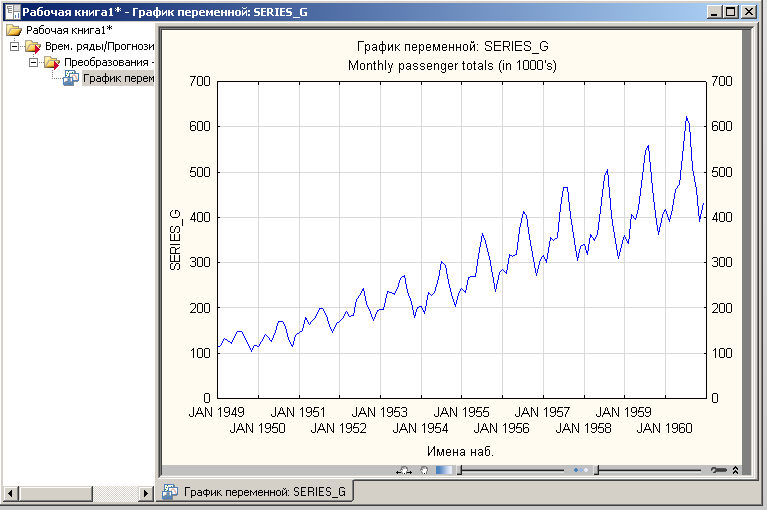
\includegraphics[height=6cm]
  {inc/Series_G/3.PNG}

  \caption{Фаза идентификации}

  \label{fig:3}
\end{figure}

\begin{center}
  \textbf{Мультипликативная сезонность}
\end{center}

% Из графика ряда также видно, что амплитуда сезонных изменений со временем увеличивается
% (т.е. есть свидетельства мультипликативной сезонности), что может смещать значения автокорреляций.
% Для стабилизации этой изменчивости будет выполнено преобразование данных в натуральный логарифм.

\begin{center}
  \textbf{Логарифмическое преобразование}
\end{center}

Преобразование переменных Series\_G > x=f(x)\\
> Преобразования > Натуральный логарифм ( x=ln(x) )\\
> OK (Преобразовать выделенную переменную)

Результат действий смотри на рисунке~\ref{fig:4}.

\begin{figure}[!h]
  \centering

  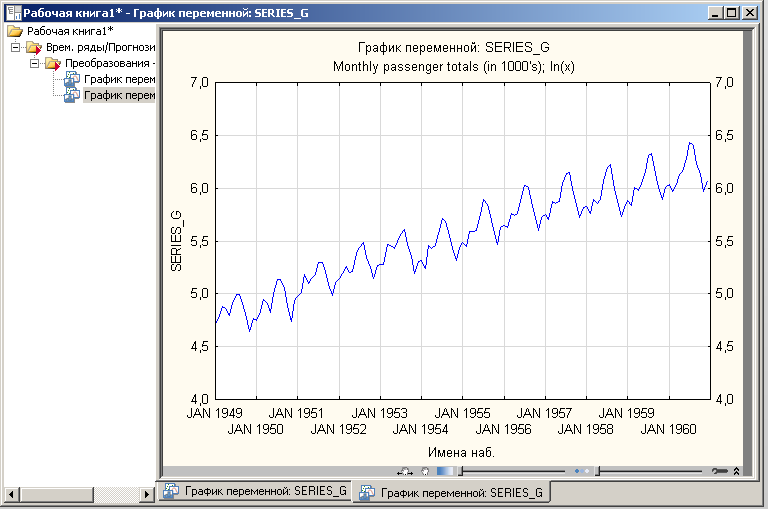
\includegraphics[height=7cm]
  {inc/Series_G/4.PNG}

  \caption{Логарифмическое преобразование}

  \label{fig:4}
\end{figure}

\begin{center}
  \textbf{Автокорреляции}
\end{center}

Преобразование переменных Series\_G > Автокорреляция\\
> Число лагов > 25\\
> Автокорреляция

Результат действий смотри на рисунке~\ref{fig:5}.

\begin{figure}[!h]
  \centering

  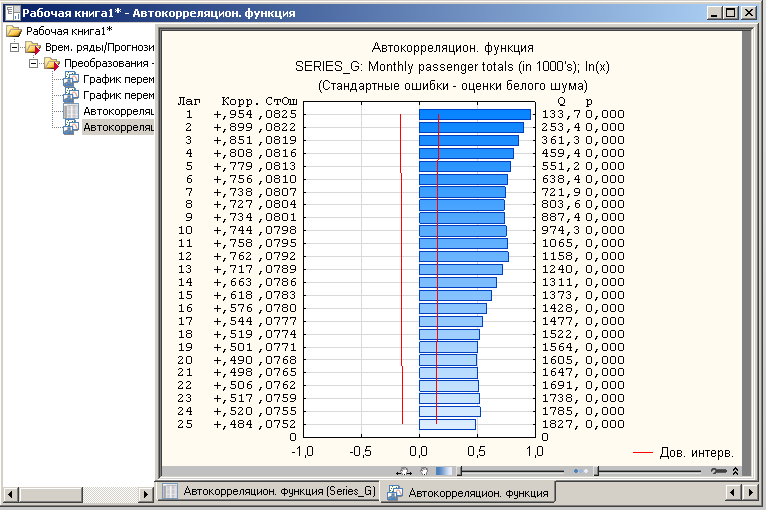
\includegraphics[height=7cm]
  {inc/Series_G/5.PNG}

  \caption{Логарифмическое преобразование}

  \label{fig:5}
\end{figure}

% = = = = = = = = = = = = = = = = = = = = = = = = = = = = = = = =

\newpage

\begin{center}
  \textbf{Разность}
\end{center}

Преобразование переменных Series\_G\\
> Разность, сумма\\
> Преобразования  > Разность ( x = x - x(лаг) )\\
> ОК (Преобразовать выделенную переменную)

Результат действий смотри на рисунке~\ref{fig:6}.

\begin{figure}[!h]
  \centering

  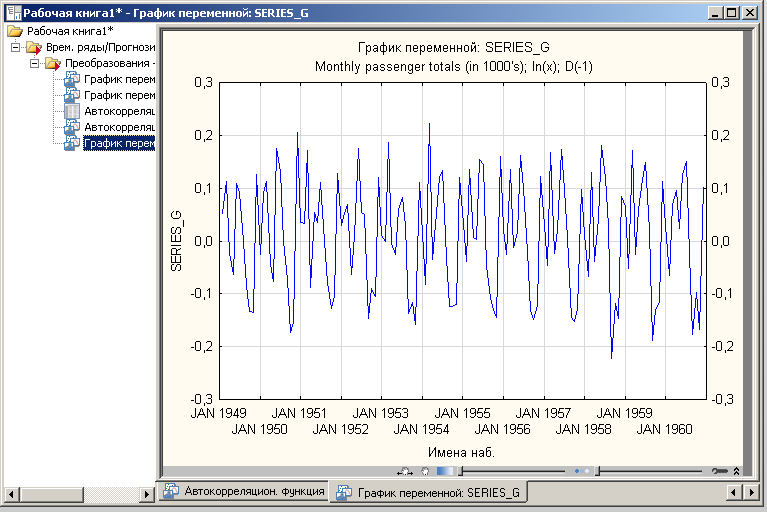
\includegraphics[height=8cm]
  {inc/Series_G/6.PNG}

  \caption{Разность}

  \label{fig:6}
\end{figure}

Преобразование переменных Series\_G\\
> Автокорреляции\\
> Автокорреляции и кросскорреляции > Автокорреляции

Результат действий смотри на рисунке~\ref{fig:7}.

\begin{figure}[!h]
  \centering

  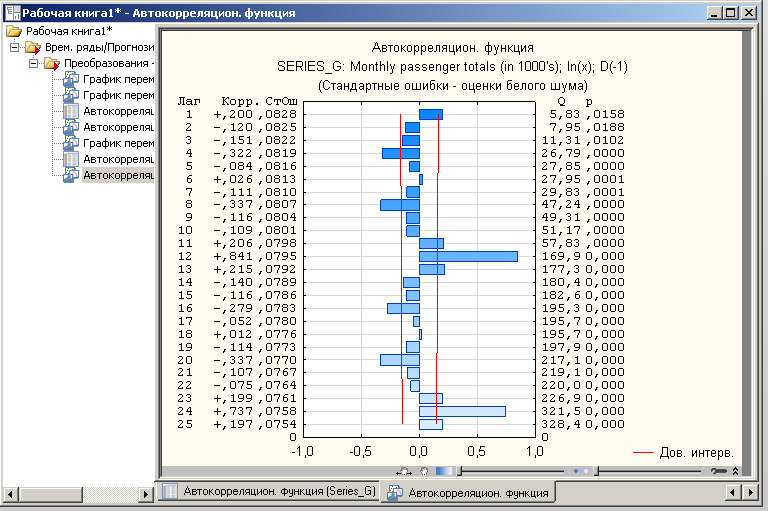
\includegraphics[height=8cm]
  {inc/Series_G/7.PNG}

  \caption{Разность}

  \label{fig:7}
\end{figure}

% = = = = = = = = = = = = = = = = = = = = = = = = = = = = = = = =

\newpage

\begin{center}
  \textbf{Сезонность}
\end{center}

\begin{center}
  \textbf{Взятие сезонной разности}
\end{center}

Преобразование переменных Series\_G\\
> Разность, сумма\\
> Преобразования  > Разность ( x = x - x(лаг) ) > Лаг=12\\
> ОК (Преобразовать выделенную переменную)

Результат действий смотри на рисунке~\ref{fig:8}.

\begin{figure}[!h]
  \centering

  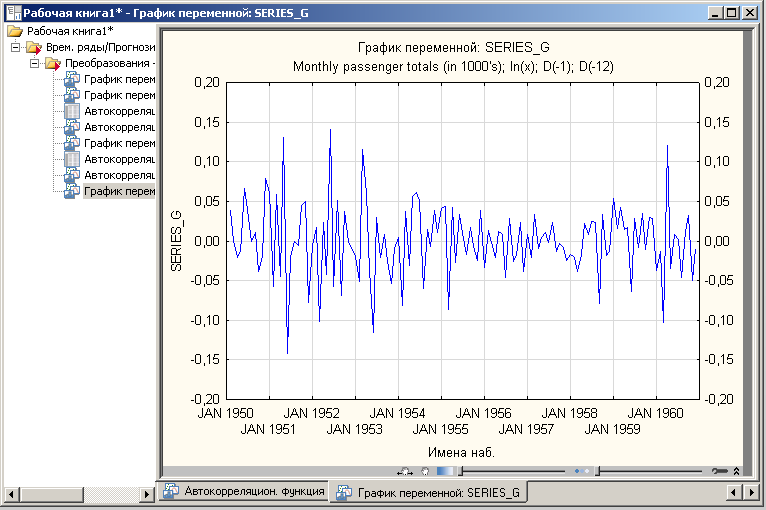
\includegraphics[height=7cm]
  {inc/Series_G/8.PNG}

  \caption{Взятие сезонной разности}

  \label{fig:8}
\end{figure}

Преобразование переменных Series\_G\\
> Графики\\
> Графики после каждого преобразования (снять галочку)\\
> Автокорреляции\\
> Автокорреляции

Результат действий смотри на рисунке~\ref{fig:9}.

\begin{figure}[!h]
  \centering

  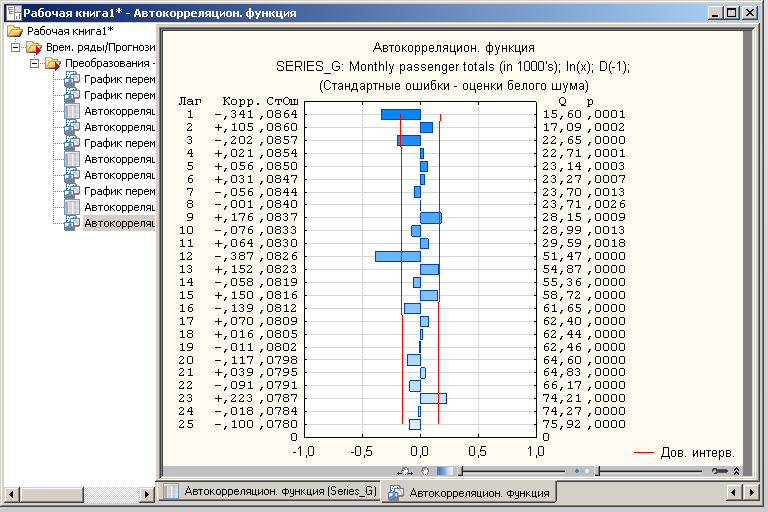
\includegraphics[height=7cm]
  {inc/Series_G/9.PNG}

  \caption{Взятие сезонной разности}

  \label{fig:9}
\end{figure}

% = = = = = = = = = = = = = = = = = = = = = = = = = = = = = = = =

\newpage

Преобразование переменных Series\_G\\
> Автокорреляции\\
> Частые Автокорреляции

Результат действий смотри на рисунке~\ref{fig:10}.

\begin{figure}[!h]
  \centering

  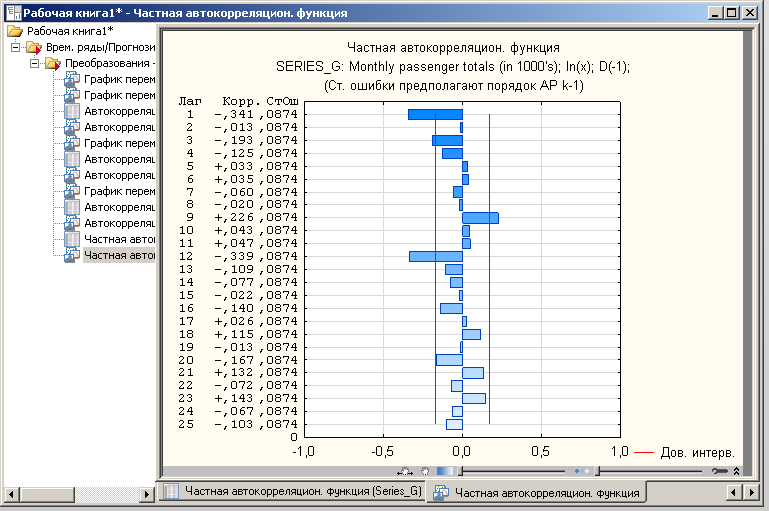
\includegraphics[height=6cm]
  {inc/Series_G/10.PNG}

  \caption{Взятие сезонной разности}

  \label{fig:10}
\end{figure}

% \begin{center}
%   \textbf{Параметры, подлежащие оценке}
% \end{center}

% Коррелограмма выглядит хорошо, и теперь ряд готов для ARIMA.
% Основываясь на изучении природы ряда (т.е. на этапе идентификации ARIMA),
% можно прийти к выводу, что сезонная АРПСС (с лагом 12)
% и несезонная модель (с лагом 1) достаточно хорошо подходят к преобразованному ряду.
% Будут оцениваться два параметра скользящего среднего модели АРПСС:
% один сезонный (Qs) и один несезонный (q).
% Параметры авторегрессии отсутствуют в модели.

\begin{center}
  \textbf{Диалог спецификаций ARIMA}
\end{center}

Преобразование переменных Series\_G\\
> Отмена\\
> L SERIES\_G Montly passenger totals (in 1000's)\\
> Методы\\
> Преобразовать переменную (ряд) перед анализом\\
> Натур. логарифм (установить флажок)\\
> Разность (установить флажок)\\
> 1. Лаг=1 > Порядок разности=1\\
> 2. Лаг=12 > Порядок разности=1\\
> q - скольз. средн.=1 > Q - Сезонных=1

Результат действий смотри на рисунке~\ref{fig:11}.

\begin{figure}[!h]
  \centering

  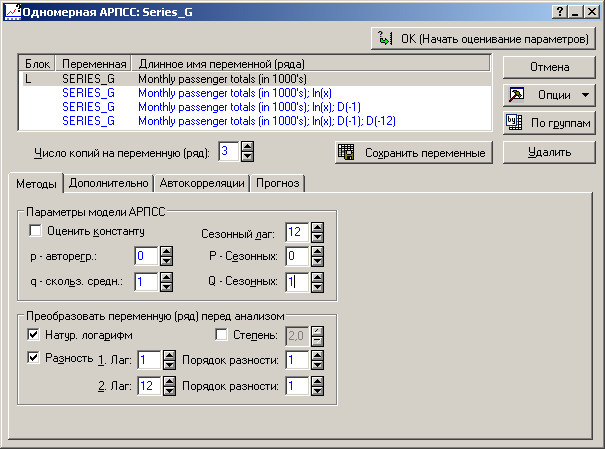
\includegraphics[height=6cm]
  {inc/Series_G/11.PNG}

  \caption{Диалог спецификаций ARIMA}

  \label{fig:11}
\end{figure}

% = = = = = = = = = = = = = = = = = = = = = = = = = = = = = = = =

\begin{center}
  \textbf{Оценивание параметров}
\end{center}

> ОК (Начать оценивание параметров)

Результат действий смотри на рисунке~\ref{fig:12}.

\begin{figure}[!h]
  \centering

  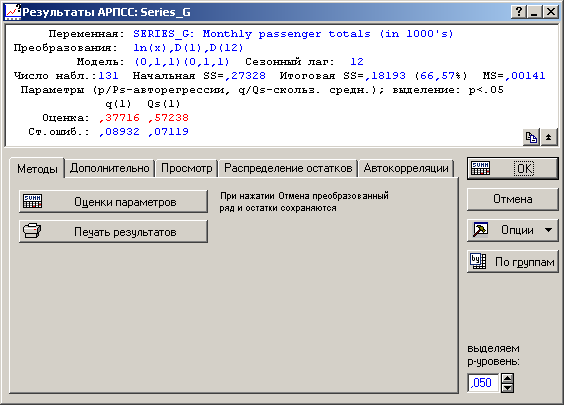
\includegraphics[height=9cm]
  {inc/Series_G/12.PNG}

  \caption{Оценивание параметров}

  \label{fig:12}
\end{figure}

\begin{center}
  \textbf{Вывод ARIMA}
\end{center}

> ОК

Результат действий смотри на рисунке~\ref{fig:13}.

\begin{figure}[!h]
  \centering

  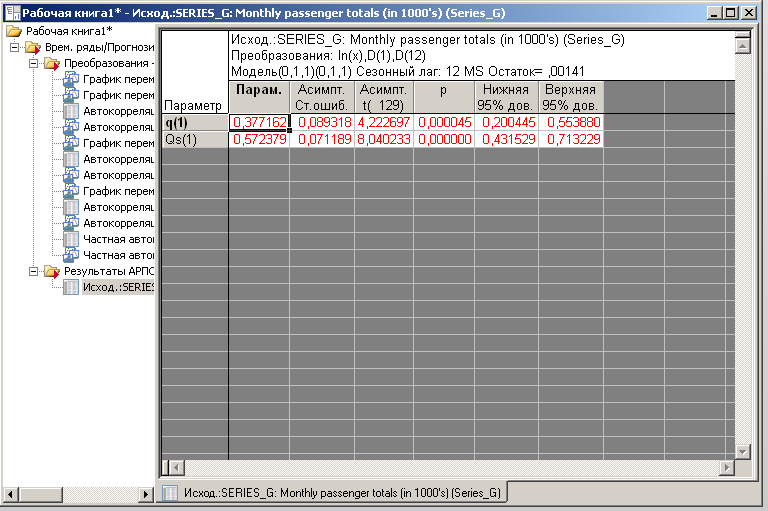
\includegraphics[height=8cm]
  {inc/Series_G/13.PNG}

  \caption{Вывод ARIMA}

  \label{fig:13}
\end{figure}

% = = = = = = = = = = = = = = = = = = = = = = = = = = = = = = = =

\newpage

\begin{center}
  \textbf{Параметры прогноза}
\end{center}

Результаты АРПСС: Series\_G
> Дополнительно > Прогноз

Результат действий смотри на рисунке~\ref{fig:14}.

\begin{figure}[!h]
  \centering

  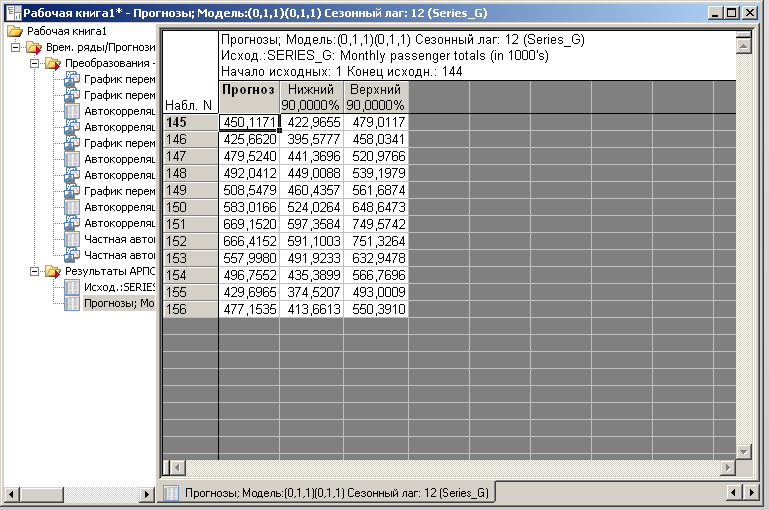
\includegraphics[height=8cm]
  {inc/Series_G/14.PNG}

  \caption{Вывод ARIMA}

  \label{fig:14}
\end{figure}

\begin{center}
  \textbf{График прогнозов}
\end{center}

Результаты АРПСС: Series\_G
> Дополнительно > График ряда и прогнозов

Результат действий смотри на рисунке~\ref{fig:15}.

\begin{figure}[!h]
  \centering

  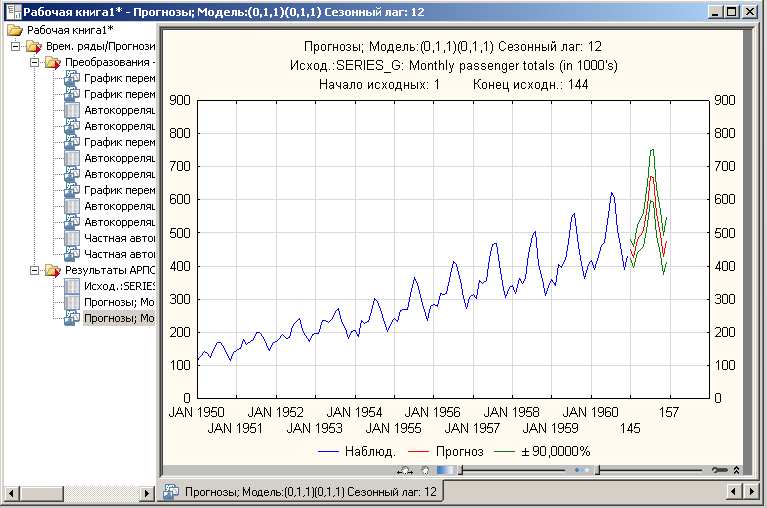
\includegraphics[height=8cm]
  {inc/Series_G/15.PNG}

  \caption{График прогнозов}

  \label{fig:15}
\end{figure}

% = = = = = = = = = = = = = = = = = = = = = = = = = = = = = = = =

\newpage

Результаты АРПСС: Series\_G\\
> Дополнительно
> Число набл.=12
> Начать с=133\\
> График ряда и прогнозов

Результат действий смотри на рисунке~\ref{fig:16}.

\begin{figure}[!h]
  \centering

  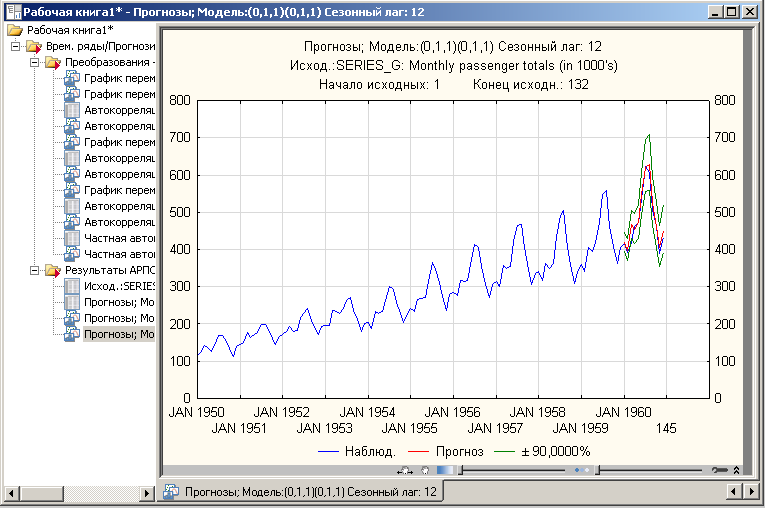
\includegraphics[height=8cm]
  {inc/Series_G/16.PNG}

  \caption{График прогнозов}

  \label{fig:16}
\end{figure}

\begin{center}
  \textbf{Графики нормальной вероятности}
\end{center}

Результаты АРПСС: Series\_G\\
> Распределение остатков
> Нормальный график

Результат действий смотри на рисунке~\ref{fig:17}.

\begin{figure}[!h]
  \centering

  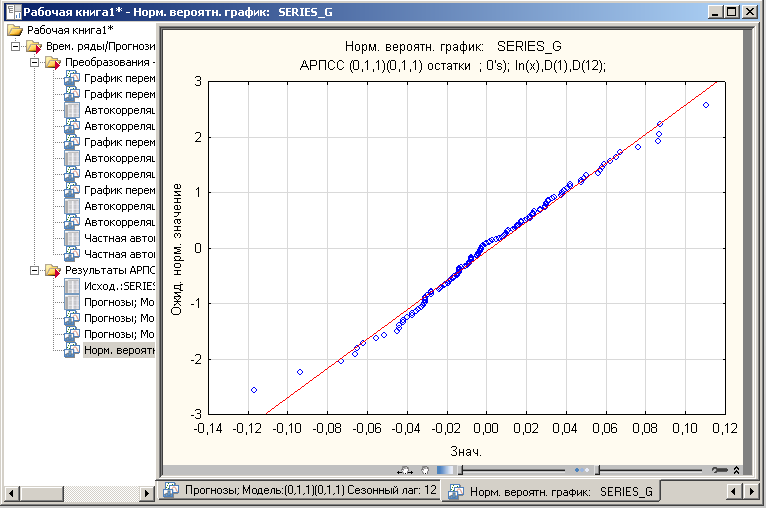
\includegraphics[height=8cm]
  {inc/Series_G/17.PNG}

  \caption{Графики нормальной вероятности}

  \label{fig:17}
\end{figure}

% = = = = = = = = = = = = = = = = = = = = = = = = = = = = = = = =

\newpage

Результаты АРПСС: Series\_G\\
> Распределение остатков
> Нормальный график без тренда

Результат действий смотри на рисунке~\ref{fig:18}.

\begin{figure}[!h]
  \centering

  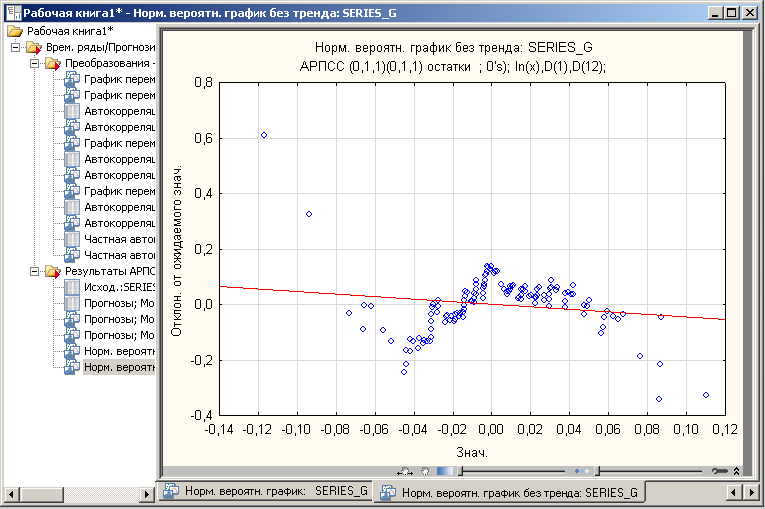
\includegraphics[height=9cm]
  {inc/Series_G/18.PNG}

  \caption{Нормальный график без тренда}

  \label{fig:18}
\end{figure}

Результаты АРПСС: Series\_G\\
> Распределение остатков
> Гистограмма

Результат действий смотри на рисунке~\ref{fig:19}.

\begin{figure}[!h]
  \centering

  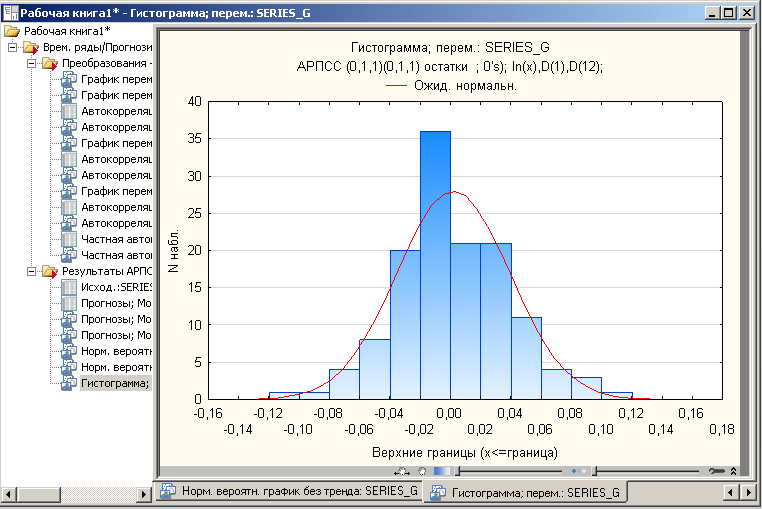
\includegraphics[height=9cm]
  {inc/Series_G/19.PNG}

  \caption{Гистограмма}

  \label{fig:19}
\end{figure}

\newpage

\begin{center}
  \textbf{Автокорреляция остатков}
\end{center}

Результаты АРПСС: Series\_G\\
> Автокорреляции
> Автокорреляции остатков
> Автокорреляции

Результат действий смотри на рисунке~\ref{fig:20}.

\begin{figure}[!h]
  \centering

  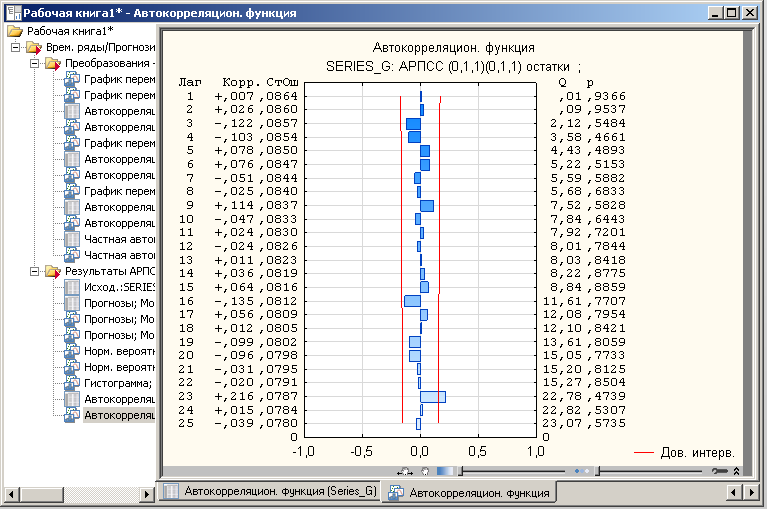
\includegraphics[height=8cm]
  {inc/Series_G/20.PNG}

  \caption{Автокорреляция остатков}

  \label{fig:20}
\end{figure}

\begin{center}
  \textbf{Дальнейшие анализы}
\end{center}

Результаты АРПСС: Series\_G > Отмена\\
> Дополнительно > Метод оценивания > Точный (Меларда)\\

Результат действий смотри на рисунке~\ref{fig:21}.

\begin{figure}[!h]
  \centering

  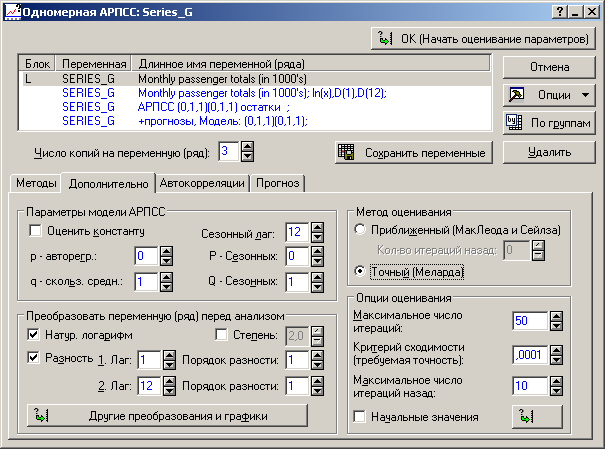
\includegraphics[height=8cm]
  {inc/Series_G/21.PNG}

  \caption{Дальнейшие анализы}

  \label{fig:21}
\end{figure}

\newpage

> Прогноз > График двух списков перем. в разных масшт.\\
> SERIES\_G: +прогнозы, Модель: (0,1.1)(0,1,1);\\
> SERIES\_G: АРПСС (0,1,1)(0,1,1) остатки;\\

Результат действий смотри на рисунке~\ref{fig:22}.

\begin{figure}[!h]
  \centering

  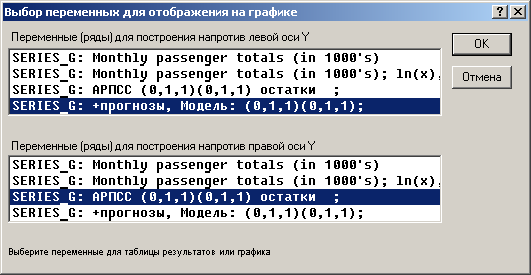
\includegraphics[height=8cm]
  {inc/Series_G/22.PNG}

  \caption{Дальнейшие анализы}

  \label{fig:22}
\end{figure}

> OK

Результат действий смотри на рисунке~\ref{fig:23}.

\begin{figure}[!h]
  \centering

  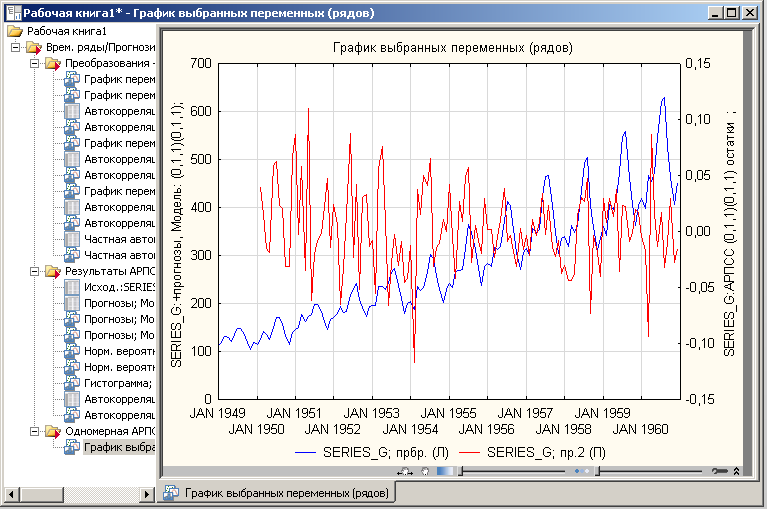
\includegraphics[height=10cm]
  {inc/Series_G/23.PNG}

  \caption{Дальнейшие анализы}

  \label{fig:23}
\end{figure}

% = = = = = = = = = = = = = = = = = = = = = = = = = = = = = = = =
% = = = = = = = = = = = = = = = = = = = = = = = = = = = = = = = =
% = = = = = = = = = = = = = = = = = = = = = = = = = = = = = = = =

\newpage

\phantomsection
\addcontentsline{toc}{section}{Вариант 2}

\begin{center}
  \textbf{Вариант 2}
\end{center}

% \phantomsection
% \addcontentsline{toc}{section}{Вариант 2}

\begin{center}
  \textbf{(Canada Gas Production)}
\end{center}

\begin{center}
  \textbf{Общие сведения}
\end{center}

Главная > Открыть > "Canada Gas Production.xlsx"\\
> Импортировать выбранный лист в Таблицу данных
> Sheet1\\
> Имена переменных из первой строки\\
> Имена наблюдений из первого столбца\\
> Импорт формата ячеек\\
> ОК

Результат действий смотри на рисунке~\ref{fig:2_1}.

\begin{figure}[!h]
  \centering

  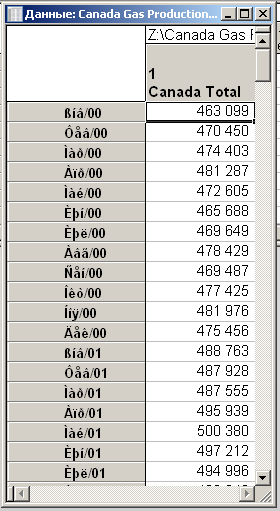
\includegraphics[height=16cm]
  {inc/Canada_Gas_Production/1.PNG}

  \caption{Общие сведения}

  \label{fig:2_1}
\end{figure}

\newpage

\begin{center}
  \textbf{Определение анализа}
\end{center}

Анализ > Углубленные методы > Временные ряды и прогнозирование\\
> Переменные > ОК\\
> Методы > АРПСС и автокорреляционные функции > Методы

Результат действий смотри на рисунке~\ref{fig:2_2}.

\begin{figure}[!h]
  \centering

  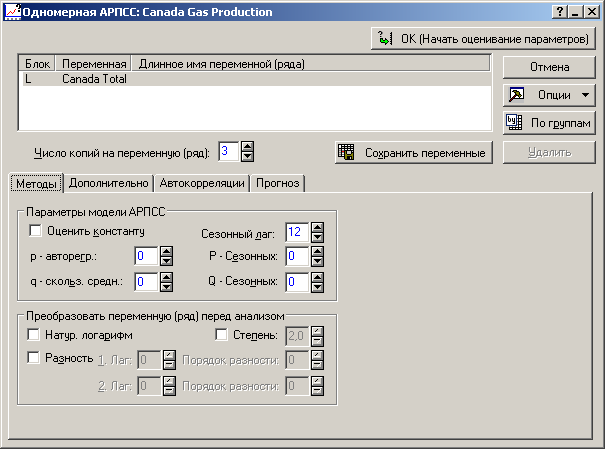
\includegraphics[height=6cm]
  {inc/Canada_Gas_Production/2.PNG}

  \caption{Определение анализа}

  \label{fig:2_2}
\end{figure}

\begin{center}
  \textbf{Фаза идентификации}
\end{center}

Анализ > Углубленные методы > Временные ряды и прогнозирование > Новый\\
> Переменные > ОК\\
> Методы > АРПСС и автокорреляционные функции > Методы \\
> Дополнительно > Другие преобразования и графики\\
> Графики\\
> Задать масштаб по оси Х (мин, знач, шаг) > 1 > 12\\
> Пометить точки по оси Х > Именами наблюдений\\
> График (рядом с кнопкой Просмотр выдел. Переменной)

Результат действий смотри на рисунке~\ref{fig:2_3}.

\begin{figure}[!h]
  \centering

  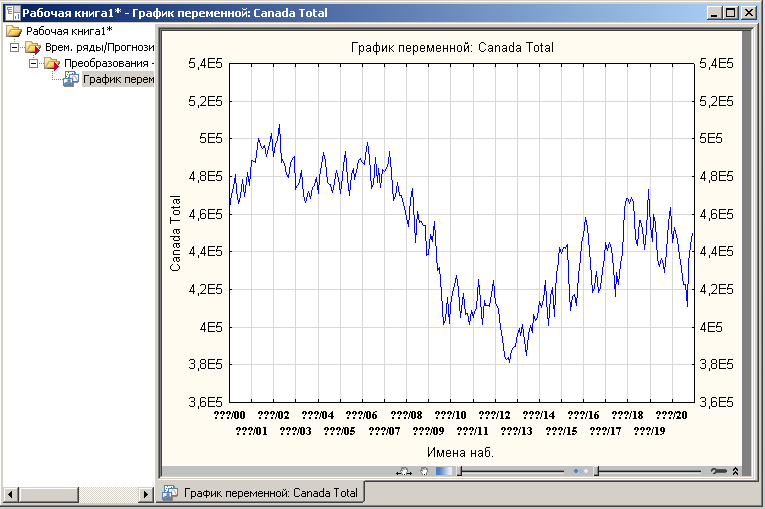
\includegraphics[height=6cm]
  {inc/Canada_Gas_Production/3.PNG}

  \caption{Фаза идентификации}

  \label{fig:2_3}
\end{figure}

\begin{center}
  \textbf{Мультипликативная сезонность}
\end{center}

% Из графика ряда также видно, что амплитуда сезонных изменений со временем увеличивается
% (т.е. есть свидетельства мультипликативной сезонности), что может смещать значения автокорреляций.
% Для стабилизации этой изменчивости будет выполнено преобразование данных в натуральный логарифм.

\begin{center}
  \textbf{Логарифмическое преобразование}
\end{center}

Преобразование переменных Series\_G > x=f(x)\\
> Преобразования > Натуральный логарифм ( x=ln(x) )\\
> OK (Преобразовать выделенную переменную)

Результат действий смотри на рисунке~\ref{fig:2_4}.

\begin{figure}[!h]
  \centering

  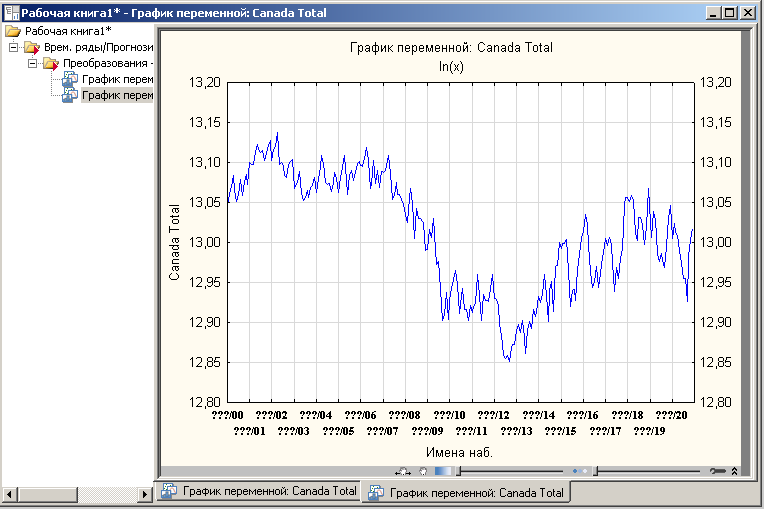
\includegraphics[height=7cm]
  {inc/Canada_Gas_Production/4.PNG}

  \caption{Логарифмическое преобразование}

  \label{fig:2_4}
\end{figure}

\begin{center}
  \textbf{Автокорреляции}
\end{center}

Преобразование переменных Series\_G > Автокорреляция\\
> Число лагов > 25\\
> Автокорреляция

Результат действий смотри на рисунке~\ref{fig:2_5}.

\begin{figure}[!h]
  \centering

  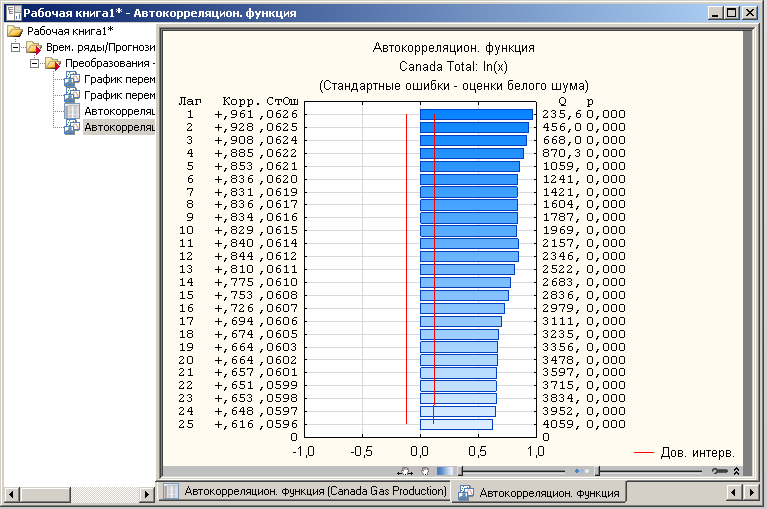
\includegraphics[height=7cm]
  {inc/Canada_Gas_Production/5.PNG}

  \caption{Логарифмическое преобразование}

  \label{fig:2_5}
\end{figure}

% = = = = = = = = = = = = = = = = = = = = = = = = = = = = = = = =

\newpage

\begin{center}
  \textbf{Разность}
\end{center}

Преобразование переменных: Canada\_Gas\_Production\\
> Разность, сумма\\
> Преобразования  > Разность ( x = x - x(лаг) )\\
> ОК (Преобразовать выделенную переменную)

Результат действий смотри на рисунке~\ref{fig:2_6}.

\begin{figure}[!h]
  \centering

  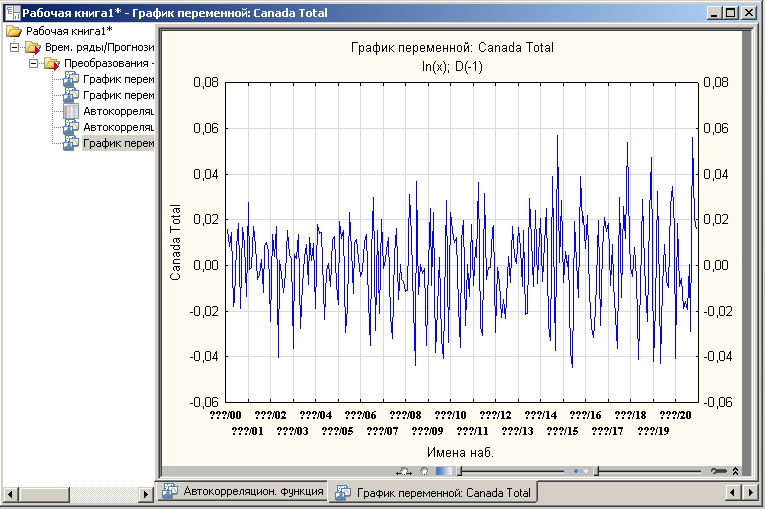
\includegraphics[height=8cm]
  {inc/Canada_Gas_Production/6.PNG}

  \caption{Разность}

  \label{fig:2_6}
\end{figure}

Преобразование переменных: Canada\_Gas\_Production\\
> Автокорреляции\\
> Автокорреляции и кросскорреляции > Автокорреляции

Результат действий смотри на рисунке~\ref{fig:2_7}.

\begin{figure}[!h]
  \centering

  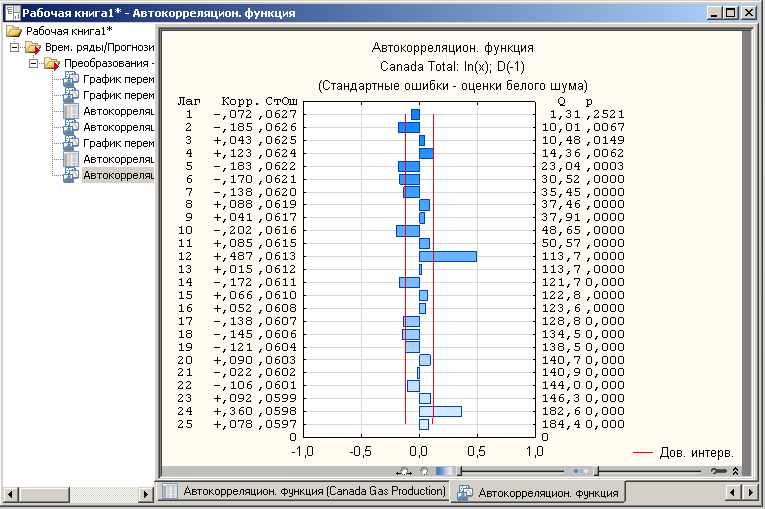
\includegraphics[height=8cm]
  {inc/Canada_Gas_Production/7.PNG}

  \caption{Разность}

  \label{fig:2_7}
\end{figure}

% = = = = = = = = = = = = = = = = = = = = = = = = = = = = = = = =

\newpage

\begin{center}
  \textbf{Сезонность}
\end{center}

\begin{center}
  \textbf{Взятие сезонной разности}
\end{center}

Преобразование переменных: Canada\_Gas\_Production\\
> Разность, сумма\\
> Преобразования  > Разность ( x = x - x(лаг) ) > Лаг=12\\
> ОК (Преобразовать выделенную переменную)

Результат действий смотри на рисунке~\ref{fig:2_8}.

\begin{figure}[!h]
  \centering

  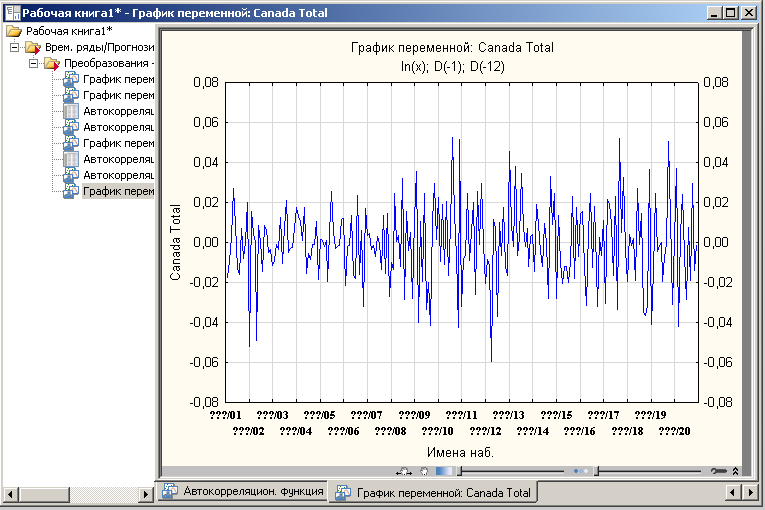
\includegraphics[height=7cm]
  {inc/Canada_Gas_Production/8.PNG}

  \caption{Взятие сезонной разности}

  \label{fig:2_8}
\end{figure}

Преобразование переменных: Canada\_Gas\_Production\\
> Графики\\
> Графики после каждого преобразования (снять галочку)\\
> Автокорреляции\\
> Автокорреляции

Результат действий смотри на рисунке~\ref{fig:2_9}.

\begin{figure}[!h]
  \centering

  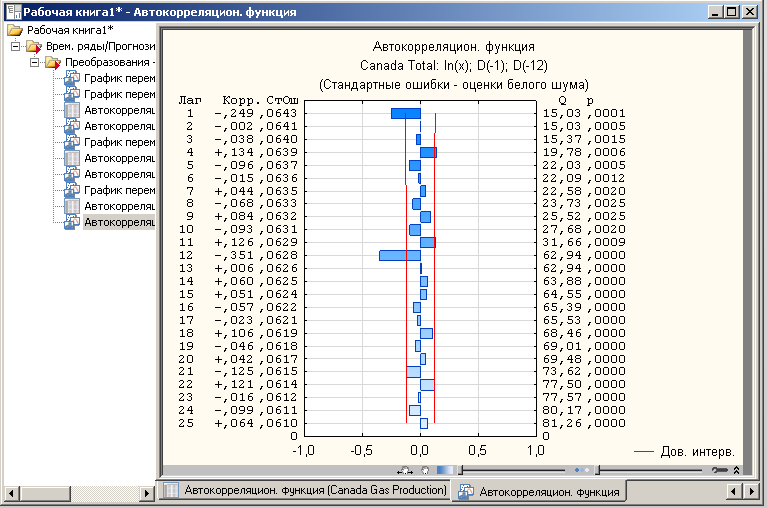
\includegraphics[height=7cm]
  {inc/Canada_Gas_Production/9.PNG}

  \caption{Взятие сезонной разности}

  \label{fig:2_9}
\end{figure}

% = = = = = = = = = = = = = = = = = = = = = = = = = = = = = = = =

\newpage

Преобразование переменных: Canada\_Gas\_Production\\
> Автокорреляции\\
> Частые Автокорреляции

Результат действий смотри на рисунке~\ref{fig:2_10}.

\begin{figure}[!h]
  \centering

  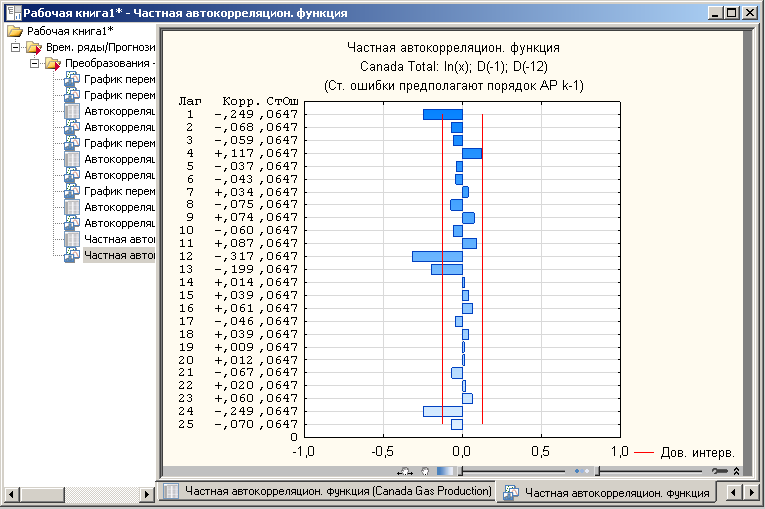
\includegraphics[height=6cm]
  {inc/Canada_Gas_Production/10.PNG}

  \caption{Взятие сезонной разности}

  \label{fig:2_10}
\end{figure}

% \begin{center}
%   \textbf{Параметры, подлежащие оценке}
% \end{center}

% Коррелограмма выглядит хорошо, и теперь ряд готов для ARIMA.
% Основываясь на изучении природы ряда (т.е. на этапе идентификации ARIMA),
% можно прийти к выводу, что сезонная АРПСС (с лагом 12)
% и несезонная модель (с лагом 1) достаточно хорошо подходят к преобразованному ряду.
% Будут оцениваться два параметра скользящего среднего модели АРПСС:
% один сезонный (Qs) и один несезонный (q).
% Параметры авторегрессии отсутствуют в модели.

\begin{center}
  \textbf{Диалог спецификаций ARIMA}
\end{center}

Преобразование переменных: Canada\_Gas\_Production\\
> Отмена\\
> L SERIES\_G Montly passenger totals (in 1000's)\\
> Методы\\
> Преобразовать переменную (ряд) перед анализом\\
> Натур. логарифм (установить флажок)\\
> Разность (установить флажок)\\
> 1. Лаг=1 > Порядок разности=1\\
> 2. Лаг=12 > Порядок разности=1\\
> q - скольз. средн.=1 > Q - Сезонных=1

Результат действий смотри на рисунке~\ref{fig:2_11}.

\begin{figure}[!h]
  \centering

  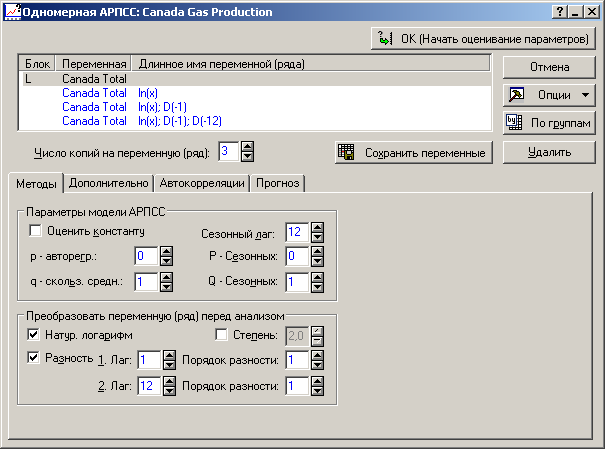
\includegraphics[height=6cm]
  {inc/Canada_Gas_Production/11.PNG}

  \caption{Диалог спецификаций ARIMA}

  \label{fig:2_11}
\end{figure}

% = = = = = = = = = = = = = = = = = = = = = = = = = = = = = = = =

\begin{center}
  \textbf{Оценивание параметров}
\end{center}

> ОК (Начать оценивание параметров)

Результат действий смотри на рисунке~\ref{fig:2_12}.

\begin{figure}[!h]
  \centering

  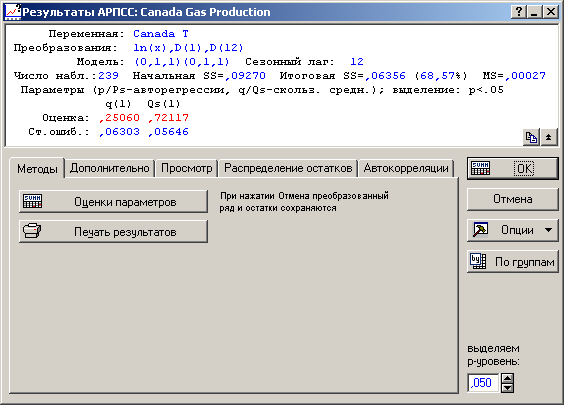
\includegraphics[height=9cm]
  {inc/Canada_Gas_Production/12.PNG}

  \caption{Оценивание параметров}

  \label{fig:2_12}
\end{figure}

\begin{center}
  \textbf{Вывод ARIMA}
\end{center}

> ОК

Результат действий смотри на рисунке~\ref{fig:2_13}.

\begin{figure}[!h]
  \centering

  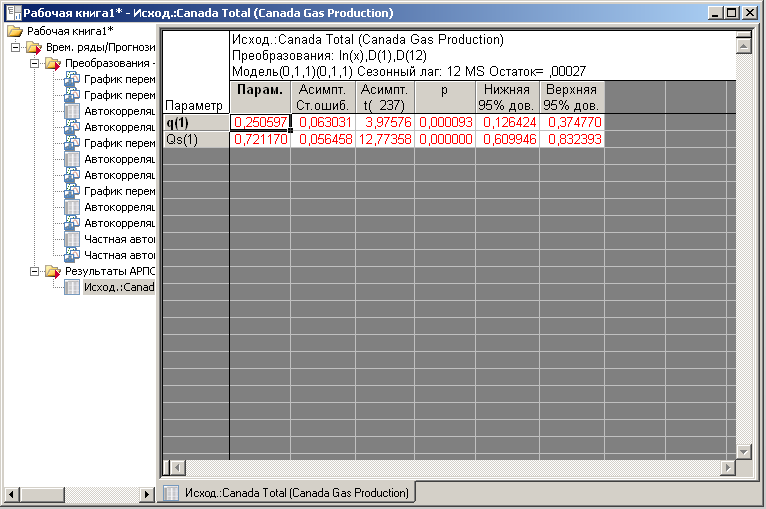
\includegraphics[height=8cm]
  {inc/Canada_Gas_Production/13.PNG}

  \caption{Вывод ARIMA}

  \label{fig:2_13}
\end{figure}

% = = = = = = = = = = = = = = = = = = = = = = = = = = = = = = = =

\newpage

\begin{center}
  \textbf{Параметры прогноза}
\end{center}

Результаты АРПСС: Canada Gas Production
> Дополнительно > Прогноз

Результат действий смотри на рисунке~\ref{fig:2_14}.

\begin{figure}[!h]
  \centering

  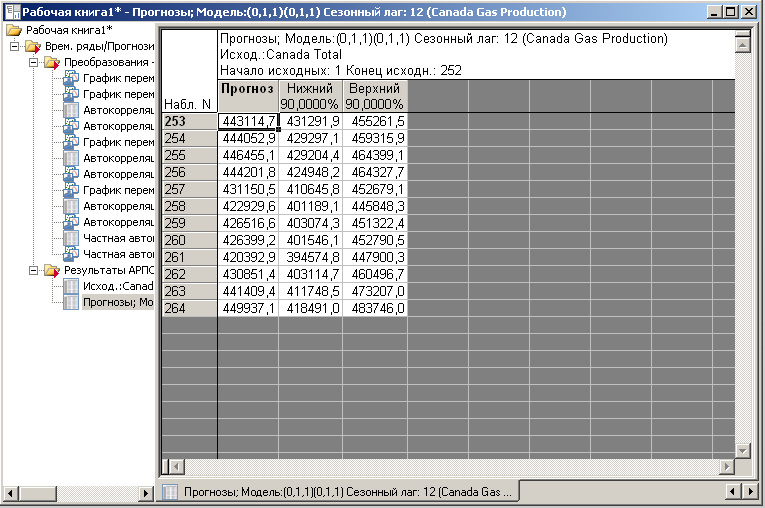
\includegraphics[height=8cm]
  {inc/Canada_Gas_Production/14.PNG}

  \caption{Вывод ARIMA}

  \label{fig:2_14}
\end{figure}

\begin{center}
  \textbf{График прогнозов}
\end{center}

Результаты АРПСС: Canada Gas Production\\
> Дополнительно > График ряда и прогнозов

Результат действий смотри на рисунке~\ref{fig:2_15}.

\begin{figure}[!h]
  \centering

  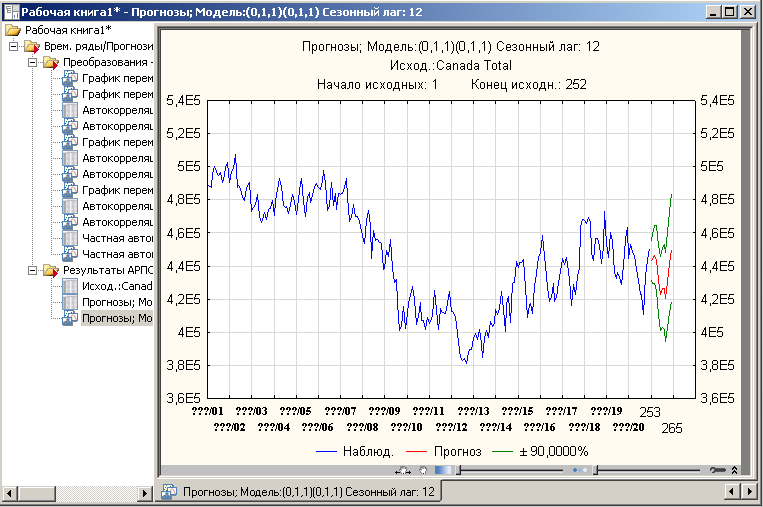
\includegraphics[height=8cm]
  {inc/Canada_Gas_Production/15.PNG}

  \caption{График прогнозов}

  \label{fig:2_15}
\end{figure}

% = = = = = = = = = = = = = = = = = = = = = = = = = = = = = = = =

\newpage

Результаты АРПСС: Canada Gas Production\\
> Дополнительно
> Число набл.=12
> Начать с=242 (253-12+1)\\
> График ряда и прогнозов

Результат действий смотри на рисунке~\ref{fig:2_16}.

\begin{figure}[!h]
  \centering

  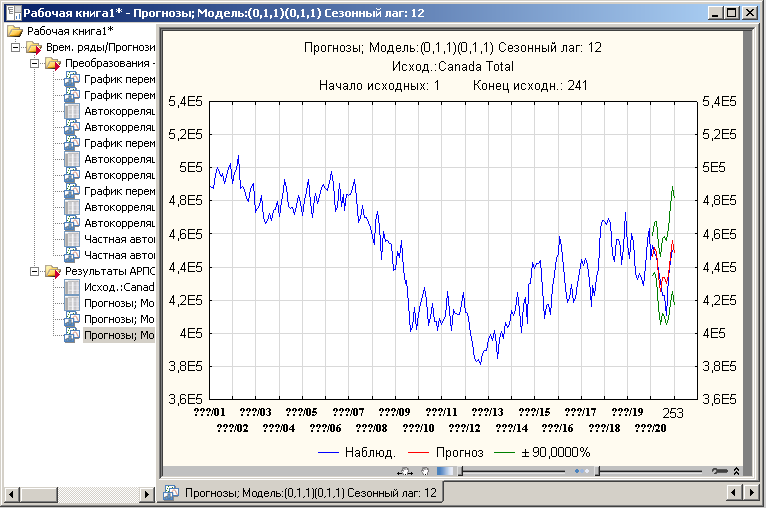
\includegraphics[height=8cm]
  {inc/Canada_Gas_Production/16.PNG}

  \caption{График прогнозов}

  \label{fig:2_16}
\end{figure}

\begin{center}
  \textbf{Графики нормальной вероятности}
\end{center}

Результаты АРПСС: Canada Gas Production\\
> Распределение остатков
> Нормальный график

Результат действий смотри на рисунке~\ref{fig:2_17}.

\begin{figure}[!h]
  \centering

  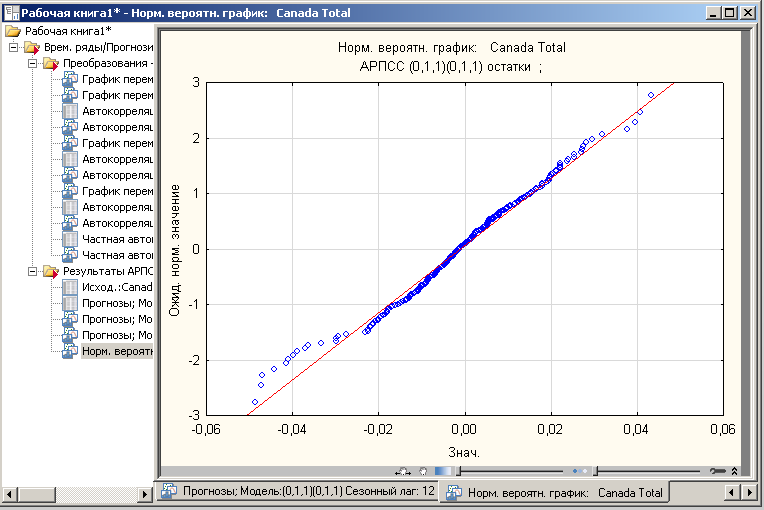
\includegraphics[height=8cm]
  {inc/Canada_Gas_Production/17.PNG}

  \caption{Графики нормальной вероятности}

  \label{fig:2_17}
\end{figure}

% = = = = = = = = = = = = = = = = = = = = = = = = = = = = = = = =

\newpage

Результаты АРПСС: Canada Gas Production\\
> Распределение остатков
> Нормальный график без тренда

Результат действий смотри на рисунке~\ref{fig:2_18}.

\begin{figure}[!h]
  \centering

  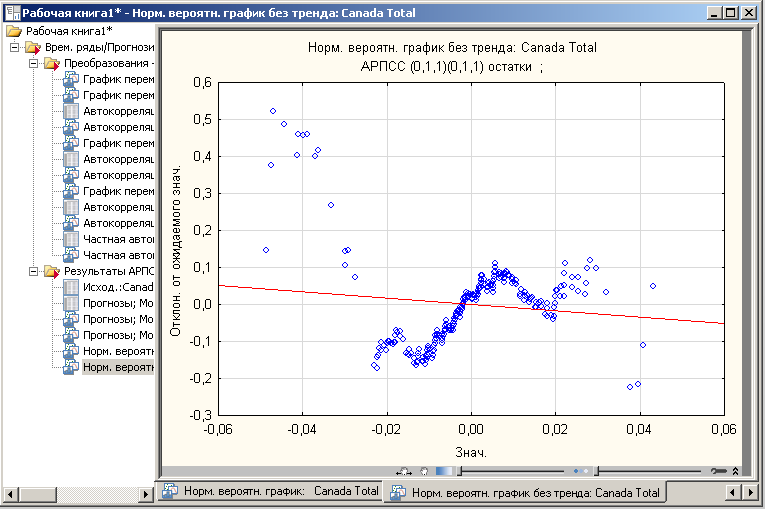
\includegraphics[height=9cm]
  {inc/Canada_Gas_Production/18.PNG}

  \caption{Нормальный график без тренда}

  \label{fig:2_18}
\end{figure}

Результаты АРПСС: Canada Gas Production\\
> Распределение остатков
> Гистограмма

Результат действий смотри на рисунке~\ref{fig:2_19}.

\begin{figure}[!h]
  \centering

  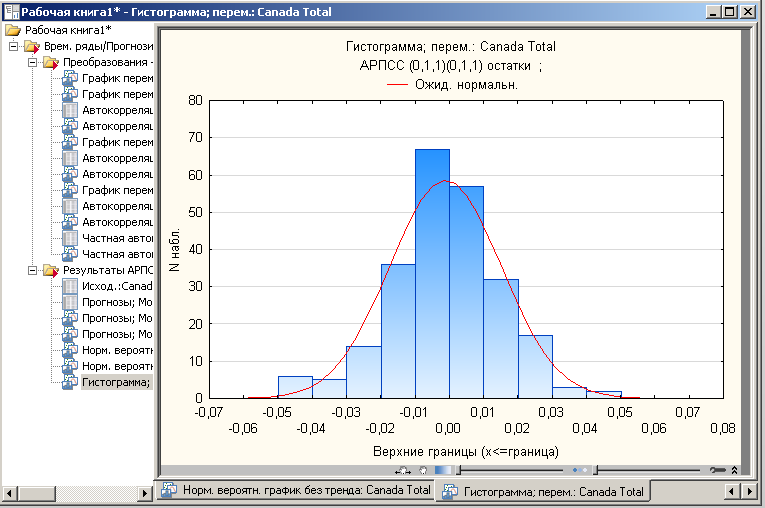
\includegraphics[height=9cm]
  {inc/Canada_Gas_Production/19.PNG}

  \caption{Гистограмма}

  \label{fig:2_19}
\end{figure}

\newpage

\begin{center}
  \textbf{Автокорреляция остатков}
\end{center}

Результаты АРПСС: Canada Gas Production\\
> Автокорреляции
> Автокорреляции остатков
> Автокорреляции

Результат действий смотри на рисунке~\ref{fig:2_20}.

\begin{figure}[!h]
  \centering

  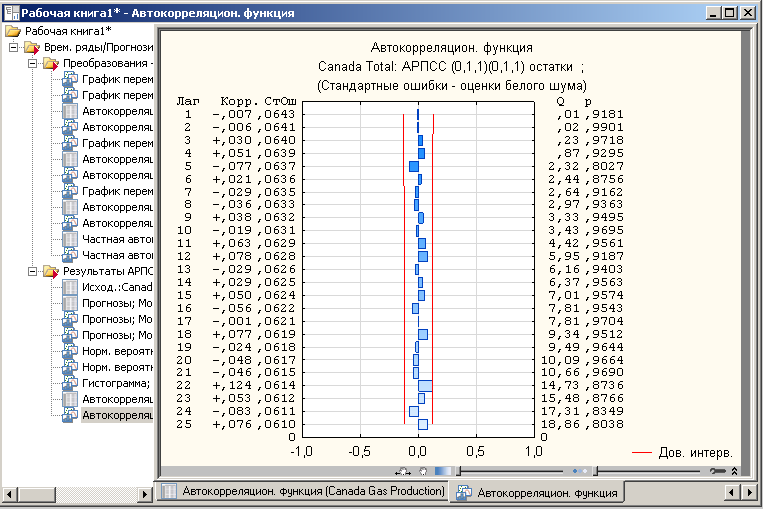
\includegraphics[height=8cm]
  {inc/Canada_Gas_Production/20.PNG}

  \caption{Автокорреляция остатков}

  \label{fig:2_20}
\end{figure}

\begin{center}
  \textbf{Дальнейшие анализы}
\end{center}

Результаты АРПСС: Canada Gas Production > Отмена\\
> Дополнительно > Метод оценивания > Точный (Меларда)\\

Результат действий смотри на рисунке~\ref{fig:2_21}.

\begin{figure}[!h]
  \centering

  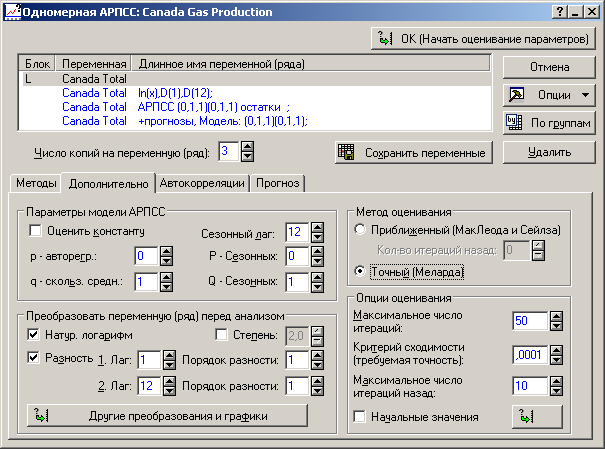
\includegraphics[height=8cm]
  {inc/Canada_Gas_Production/21.PNG}

  \caption{Дальнейшие анализы}

  \label{fig:2_21}
\end{figure}

\newpage

> Прогноз > График двух списков перем. в разных масшт.\\
> SERIES\_G: +прогнозы, Модель: (0,1.1)(0,1,1);\\
> SERIES\_G: АРПСС (0,1,1)(0,1,1) остатки;\\

Результат действий смотри на рисунке~\ref{fig:2_22}.

\begin{figure}[!h]
  \centering

  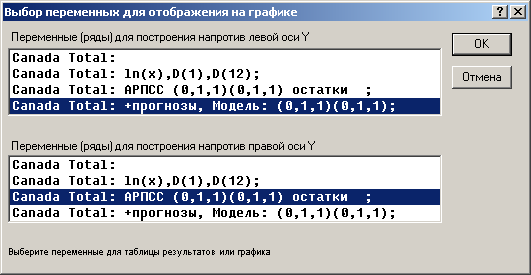
\includegraphics[height=8cm]
  {inc/Canada_Gas_Production/22.PNG}

  \caption{Дальнейшие анализы}

  \label{fig:2_22}
\end{figure}

> OK

Результат действий смотри на рисунке~\ref{fig:2_23}.

\begin{figure}[!h]
  \centering

  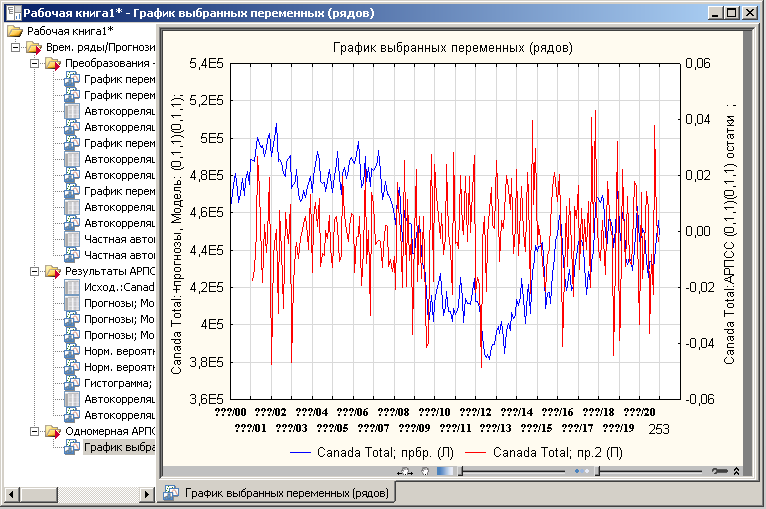
\includegraphics[height=10cm]
  {inc/Canada_Gas_Production/23.PNG}

  \caption{Дальнейшие анализы}

  \label{fig:2_23}
\end{figure}
